\documentclass[tikz, border=4pt]{standalone}
\usepackage[T1]{fontenc}
\usepackage{lmodern}
\usetikzlibrary{positioning, calc, fit, backgrounds, arrows.meta, shapes.callouts, decorations.pathreplacing}

% The strength-of-evidence workflow (Methods, "Modernization policies and the
% review of their benefits"). Step 1: a review page with one cited claim. Step
% 2: the claim as the LLM (fable-5-1) returns it, with its citation resolved to
% a paper. Step 3: the extraction scaled to the 155 reviews. Step 4: the sample
% of cited papers (census of the eight least documented functions, 30 per cell
% of the four most documented). Step 5: the human rating. Numbers from
% code/63, code/67, code/68 and the retrieval manifest (code/69-70).

\definecolor{leg}{HTML}{2166ac}
\definecolor{irr}{HTML}{b2182b}
\definecolor{band}{HTML}{dbe6f2}
\definecolor{pale}{HTML}{f3f3f3}

\begin{document}
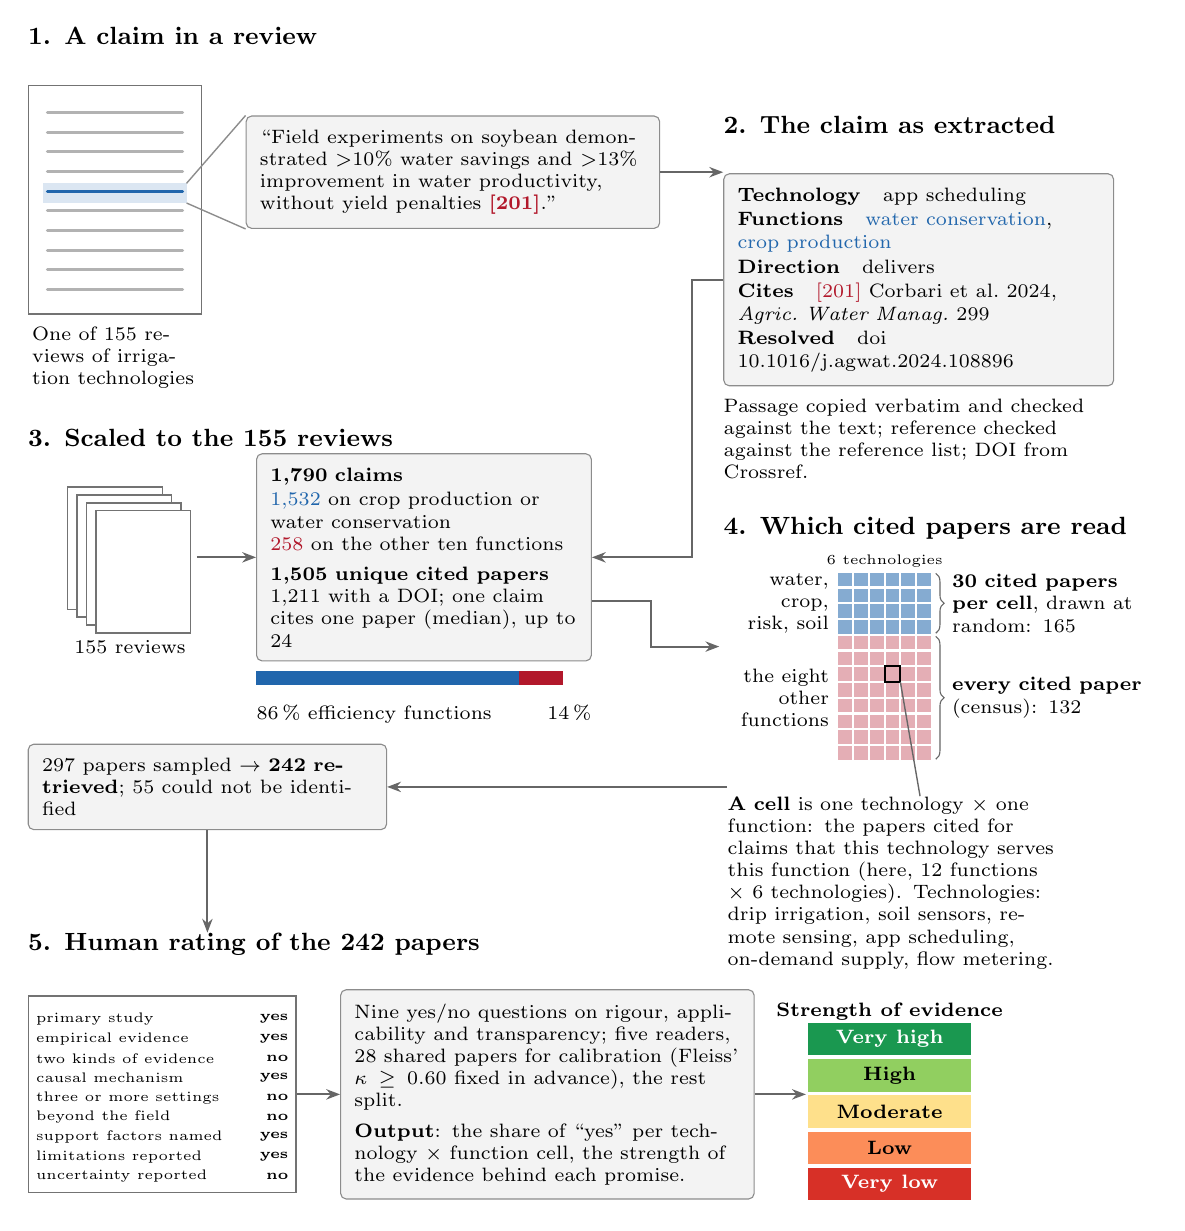
\begin{tikzpicture}[
  font=\footnotesize,
  stp/.style={font=\bfseries\small, anchor=north west, inner sep=0pt},
  note/.style={font=\scriptsize, align=left, inner sep=0pt},
  page/.style={draw=black!55, fill=white, line width=0.5pt, minimum width=2.2cm, minimum height=2.9cm, inner sep=0pt},
  line/.style={black!30, line width=1.1pt, line cap=round},
  card/.style={draw=black!45, fill=pale, rounded corners=2pt, inner sep=5pt, align=left, font=\scriptsize},
  arr/.style={-{Stealth[length=5pt]}, black!60, line width=0.7pt},
  cell/.style={draw=white, line width=0.6pt, minimum size=5.5pt, inner sep=0pt},
]

% ---------------------------------------------------------------------------
% Step 1: a review page with one cited claim
% ---------------------------------------------------------------------------
\node[stp] (s1) at (0, 0) {1. A claim in a review};
\node[page, below=5mm of s1.south west, anchor=north west] (pg) {};
\foreach \y in {0.35, 0.6, 0.85, 1.1, 1.6, 1.85, 2.1, 2.35, 2.6} {
  \draw[line] ($(pg.north west)+(0.25, -\y)$) -- ($(pg.north east)+(-0.25, -\y)$);
}
\fill[band] ($(pg.north west)+(0.2, -1.25)$) rectangle ($(pg.north east)+(-0.2, -1.5)$);
\draw[line, leg] ($(pg.north west)+(0.25, -1.35)$) -- ($(pg.north east)+(-0.25, -1.35)$);
\node[note, text width=2.1cm, anchor=north west] at ($(pg.south west)+(0.05, -0.15)$)
  {One of 155 reviews of irrigation technologies};
\node[card, text width=4.9cm, anchor=west] (quote) at ($(pg.east)+(0.55, 0.35)$)
  {``Field experiments on soybean demonstrated $>$10\% water savings and $>$13\% improvement in water productivity, without yield penalties~{\color{irr}\textbf{[201]}}.''};
\draw[black!45, line width=0.5pt] ($(pg.north east)+(-0.2, -1.5)$) -- (quote.south west);
\draw[black!45, line width=0.5pt] ($(pg.north east)+(-0.2, -1.25)$) -- (quote.north west);

% ---------------------------------------------------------------------------
% Step 2: the claim as extracted, its citation resolved
% ---------------------------------------------------------------------------
\node[stp, anchor=north west] (s2) at ($(quote.north east)+(0.8, 0)$) {2. The claim as extracted};
\node[card, text width=4.6cm, below=5mm of s2.south west, anchor=north west] (rec) {%
  \textbf{Technology}\quad app scheduling\\[1pt]
  \textbf{Functions}\quad {\color{leg}water conservation}, {\color{leg}crop production}\\[1pt]
  \textbf{Direction}\quad delivers\\[1pt]
  \textbf{Cites}\quad {\color{irr}[201]} Corbari et al.\ 2024, \textit{Agric.\ Water Manag.}\ 299\\[1pt]
  \textbf{Resolved}\quad doi 10.1016/j.agwat.2024.108896};
\node[note, text width=4.6cm, anchor=north west] (rnote) at ($(rec.south west)+(0, -0.15)$)
  {Passage copied verbatim and checked against the text; reference checked against the reference list; DOI from Crossref.};
\draw[arr] (quote.east) -- ($(rec.west |- quote.east)$);

% ---------------------------------------------------------------------------
% Step 3: scaled to 155 reviews
% ---------------------------------------------------------------------------
\node[stp, anchor=north west] (s3) at ($(s1.north west)+(0, -5.1)$) {3. Scaled to the 155 reviews};
\foreach \i in {0, 1, 2, 3} {
  \node[page, minimum width=1.2cm, minimum height=1.55cm, anchor=north west]
    at ($(s3.south west)+(0.5 + 0.12*\i, -0.5 - 0.1*\i)$) {};
}
\node[note, text width=1.6cm, align=center, anchor=north] at ($(s3.south west)+(1.3, -2.45)$) {155 reviews};
\node[card, text width=3.9cm, anchor=west] (counts) at ($(s3.south west)+(2.9, -1.4)$) {%
  \textbf{1,790 claims}\\[1pt]
  {\color{leg}1,532} on crop production or water conservation\\
  {\color{irr}258} on the other ten functions\\[3pt]
  \textbf{1,505 unique cited papers}\\
  1,211 with a DOI; one claim cites one paper (median), up to 24};
\draw[arr] ($(s3.south west)+(2.15, -1.4)$) -- (counts.west);
% share bar
\draw[fill=leg, draw=none] ($(counts.south west)+(0, -0.3)$) rectangle ++(3.34, 0.18);
\draw[fill=irr, draw=none] ($(counts.south west)+(3.34, -0.3)$) rectangle ++(0.56, 0.18);
\node[note, anchor=north west] at ($(counts.south west)+(0, -0.55)$) {86\,\% efficiency functions};
\node[note, anchor=north east] at ($(counts.south east)+(0, -0.55)$) {14\,\%};

% ---------------------------------------------------------------------------
% Step 4: which cited papers are read
% ---------------------------------------------------------------------------
\node[stp, anchor=north west] (s4) at ($(s2.north west)+(0, -5.1)$) {4. Which cited papers are read};
% grid: 12 functions (rows) x 6 technologies (columns); 4 thick rows sampled, 8 thin rows census
\begin{scope}[shift={($(s4.south west)+(1.55, -0.5)$)}]
  \foreach \r in {0, 1, 2, 3} {
    \foreach \c in {0, ..., 5} {
      \node[cell, fill=leg!55] at (\c*0.2, -\r*0.2) {};
    }
  }
  \foreach \r in {4, ..., 11} {
    \foreach \c in {0, ..., 5} {
      \node[cell, fill=irr!35] at (\c*0.2, -\r*0.2) {};
    }
  }
  \node[note, anchor=east, text width=1.4cm, align=right] at (-0.2, -0.3) {water, crop, risk, soil};
  \node[note, anchor=east, text width=1.4cm, align=right] at (-0.2, -1.5) {the eight other functions};
  \node[note, anchor=south, font=\tiny] at (0.5, 0.15) {6 technologies};
  % one cell singled out: a technology x function pair
  \draw[black, line width=0.7pt] (0.6-0.1, -1.2-0.1) rectangle (0.6+0.1, -1.2+0.1);
  \draw[black!60, line width=0.5pt] (0.7, -1.3) -- (0.95, -2.75);
  \node[note, anchor=north west, text width=4.2cm] (cnote) at (-1.5, -2.75)
    {\textbf{A cell} is one technology $\times$ one function: the papers cited for claims that this technology serves this function (here, 12 functions $\times$ 6 technologies). Technologies: drip irrigation, soil sensors, remote sensing, app scheduling, on-demand supply, flow metering.};
  \draw[decorate, decoration={brace, amplitude=3pt}, black!60] (1.15, 0.08) -- (1.15, -0.68);
  \node[note, anchor=west, text width=2.6cm] at (1.35, -0.3) {\textbf{30 cited papers per cell}, drawn at random: 165};
  \draw[decorate, decoration={brace, amplitude=3pt}, black!60] (1.15, -0.72) -- (1.15, -2.28);
  \node[note, anchor=west, text width=2.6cm] at (1.35, -1.5) {\textbf{every cited paper} (census): 132};
\end{scope}
\node[card, text width=4.2cm, anchor=north west] (samp) at ($(s3.north west)+(0, -4.0)$) {%
  297 papers sampled $\rightarrow$ \textbf{242 retrieved}; 55 could not be identified};

% ---------------------------------------------------------------------------
% Step 5: human rating
% ---------------------------------------------------------------------------
\node[stp, anchor=north west] (s5) at ($(s3.north west)+(0, -6.4)$) {5. Human rating of the 242 papers};
\node[page, minimum width=3.4cm, minimum height=2.5cm, below=5mm of s5.south west, anchor=north west] (sheet) {};
\foreach \y/\lab/\ans in {0.3/primary study/yes, 0.55/empirical evidence/yes, 0.8/two kinds of evidence/no, 1.05/causal mechanism/yes, 1.3/three or more settings/no, 1.55/beyond the field/no, 1.8/support factors named/yes, 2.05/limitations reported/yes, 2.3/uncertainty reported/no} {
  \node[note, anchor=west, font=\tiny] at ($(sheet.north west)+(0.1, -\y)$) {\lab};
  \node[note, anchor=east, font=\tiny\bfseries] at ($(sheet.north east)+(-0.1, -\y)$) {\ans};
}
\node[card, text width=4.9cm, anchor=west] (rate) at ($(sheet.east)+(0.55, 0)$) {%
  Nine yes/no questions on rigour, applicability and transparency; five readers, 28 shared papers for calibration (Fleiss' $\kappa \geq 0.60$ fixed in advance), the rest split.\\[3pt]
  \textbf{Output}: the share of ``yes'' per technology $\times$ function cell, the strength of the evidence behind each promise.};
\draw[arr] (sheet.east) -- (rate.west);
% the five-level scale the ratings are summarised into, green on top
\definecolor{lk5}{HTML}{1a9850}
\definecolor{lk4}{HTML}{91cf60}
\definecolor{lk3}{HTML}{fee08b}
\definecolor{lk2}{HTML}{fc8d59}
\definecolor{lk1}{HTML}{d73027}
\foreach \i/\lab/\col/\txt in {0/Very high/lk5/white, 1/High/lk4/black, 2/Moderate/lk3/black, 3/Low/lk2/black, 4/Very low/lk1/white} {
  \node[draw=white, line width=0.8pt, fill=\col, text=\txt, font=\scriptsize\bfseries,
        minimum width=2.1cm, minimum height=0.44cm, inner sep=0pt, anchor=north west]
    (lk\i) at ($(rate.north east)+(0.65, -0.4 - 0.46*\i)$) {\lab};
}
\node[note, anchor=south, font=\scriptsize\bfseries] at (lk0.north) {Strength of evidence};
\draw[arr] (rate.east) -- (rate.east -| lk2.west);

% flow between the steps
\draw[arr] (rec.west) -- ++(-0.4, 0) |- (counts.east);
\draw[arr] ($(counts.east)+(0, -0.55)$) -- ++(0.75, 0) |- ($(s4.south west)+(-0.05, -1.35)$);
\draw[arr] (cnote.west |- samp.east) -- (samp.east);
\draw[arr] (samp.south) -- (s5.north -| samp.south);
\end{tikzpicture}
\end{document}
